% !TEX program = xelatex
\documentclass[oneside]{article}

\title{%
\textbf{Vintage Rent}  \\
\large Documentatie \\
(Programare Avansata pe Obiecte)}
\date{}
\author{Dinu Florin-Silviu \\ grupa 231}

\makeatletter
\renewcommand{\@seccntformat}[1]{}
\makeatother

\usepackage{tikz}
\usepackage{forest}
\usepackage{hyperref}
\usepackage{amsthm}
\usepackage{amssymb}
\usepackage[romanian]{babel}
\usepackage[a4paper, margin=3cm]{geometry}
\usepackage{enumitem}
\usepackage{listings}
\usepackage{fontspec}
\usepackage{xcolor}
\usepackage{textcomp}
\usepackage{graphicx}
\usepackage{tabularx}
\usepackage{titlesec}
\usepackage{mathtools}
\usepackage{bookmark}
\usepackage{lmodern}
\usepackage{float}

\setmainfont{Roboto}

\graphicspath{ {./img/} }


\lstset{
%  tabsize=4,
extendedchars=true,
        % %upquote=false,
        % aboveskip=\baselineskip,
        columns=fixed,
        showstringspaces=false,
        extendedchars=true,
        breaklines=true,
        % prebreak = \raisebox{0ex}[0ex][0ex]{\ensuremath{\hookleftarrow}},
        showtabs=false,
        showspaces=false,
        identifierstyle=\ttfamily,
        keywordstyle=\color[rgb]{0,0,1},
        commentstyle=\color[rgb]{0.133,0.545,0.133},
        stringstyle=\color[rgb]{0.627,0.126,0.941},
        % language=Java
        frame=lines,
        literate=%
    {€}{\euro}1%
    {§}{\S}1%
    {°}{\textdegree{}}1%
    {ä}{{\"a}}1%
    {ö}{{\"o}}1%
    {ü}{{\"u}}1%
    {ß}{{\ss}}1%
    {Ä}{{\"A}}1%
    {Ö}{{\"O}}1%
    {Ü}{{\"U}}1%
    {µ}{\textmu}1%
    {¹}{{\textsuperscript{1}}}1%
    {²}{{\textsuperscript{2}}}1%
    {³}{{\textsuperscript{3}}}1%
    {¼}{\textonequarter}1%
    {½}{\textonehalf}1%
    {¢}{\textcent}1%
}

\lstdefinelanguage{pom}
{
  morestring=[b]",
  morestring=[s]{>}{<},
  morecomment=[s]{<?}{?>},
  stringstyle=\color{black},
  identifierstyle=\color{darkblue},
  keywordstyle=\color{cyan},
  morekeywords={dependency, groupId, artifactId, version}
}


\begin{document}
\pagenumbering{gobble}
\maketitle
\tableofcontents

\newpage
\pagenumbering{arabic}

\section[Introducere]{Introducere}
\paragraph{} Aplicatia permite gestionarea unui magazin care inchiriaza camere vintage. Avem utilizatori care pot fi angajati, clienti sau administratori de site. Acestora le sunt puse la dispozitie camere de diverse tipuri si obiective. Ei pot alege sa inchirieze oricare pereche de camera si obiectiv doresc. Daca apar probleme, angajatii pot adauga penalizari inchirierii.

\paragraph{}Ca o prima idee despre ce si cum se poate face, atasez diagrama relationala a bazei de date. Proiectul a fost gandit pentru un anumit workflow care este implementat si in aplicatia Java.

\begin{figure}[ht]
    \centering
    \noindent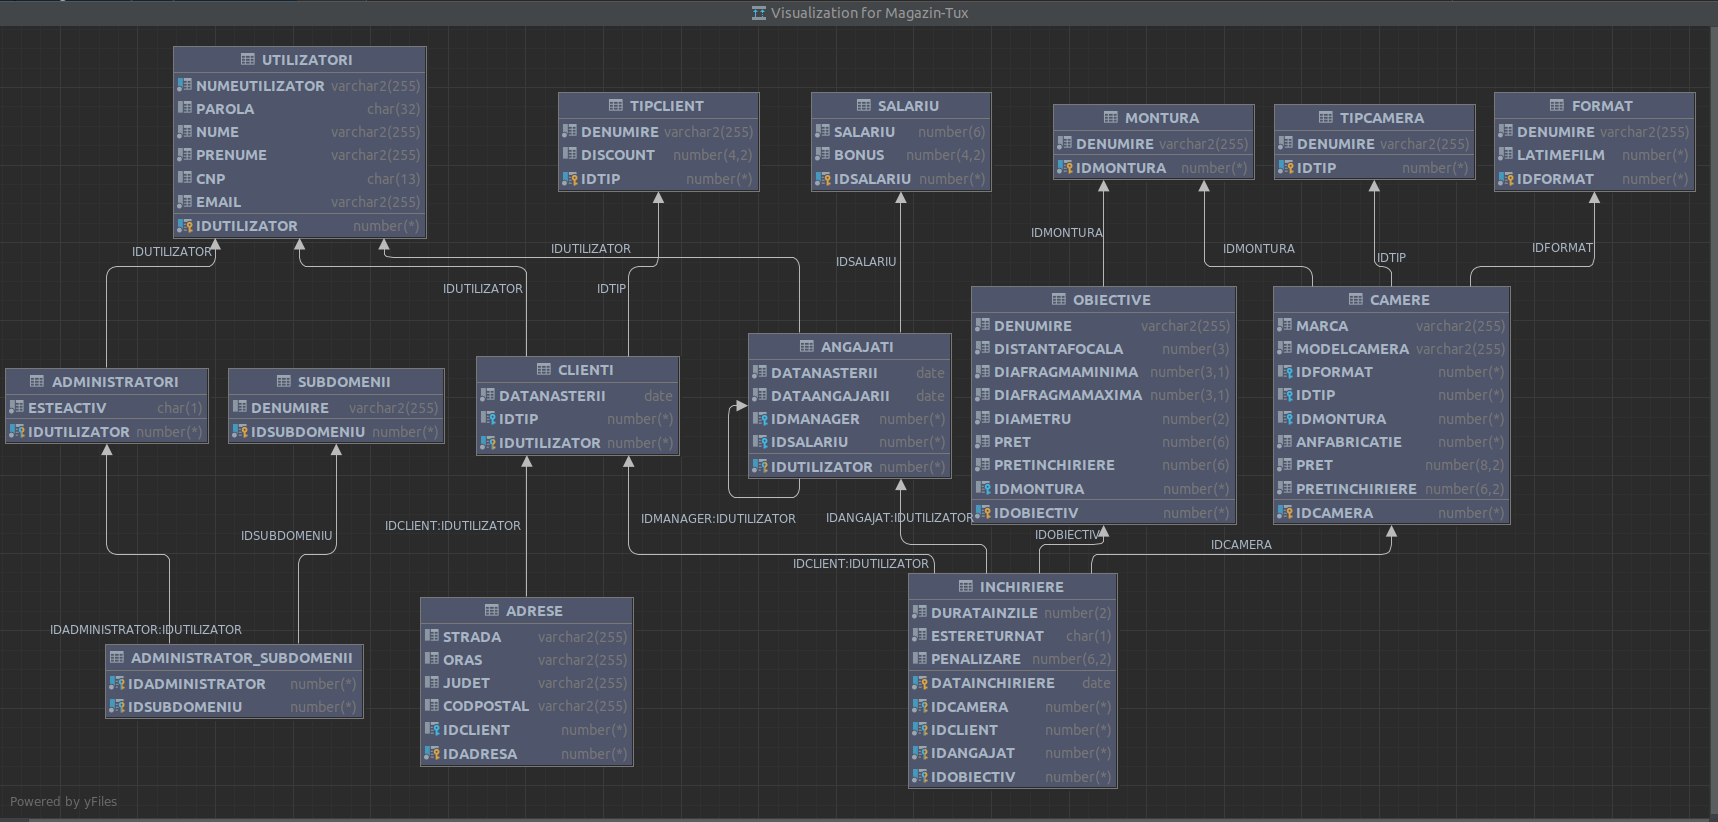
\includegraphics[width=\linewidth]{diagrama.png}
    \caption{Diagrama relationala}
    \label{fig:diagrama}
\end{figure}

\paragraph{} Pentru conexiunea la baza de date Oracle, va trebui sa intrati in folderul \textbf{docker\_oracle\_21c} si sa rulati \textbf{docker-compose up} 

\paragraph{Pe Linux} datele de conectare sunt urmatoarele:
\begin{itemize}
    \item host: 172.21.128.2
    \item port: 1521
    \item SID: ORCLCDB
    \item user: SYSTEM
    \item parola: fmilove
\end{itemize}

\paragraph{Pe Windows} datele de conectare sunt urmatoarele:
\begin{itemize}
    \item host: 0.0.0.0
    \item port: 1521
    \item SID: ORCLCDB
    \item user: SYSTEM
    \item parola: fmilove
\end{itemize}

\paragraph{}Dupa aceea rulati comenzile urmatoare pentru a crea userul folosit de program:

\begin{center}
    \begin{lstlisting}[language=sql]
        CREATE USER C##TUX IDENTIFIED BY "fmilove";
        GRANT ALL PRIVILEGES TO C##TUX;
    \end{lstlisting}
\end{center}

\paragraph{} Motivul pentru care acest utilizator exista, este ca sa nu se faca niciodata conexiunea cu SYSTEM sau alt utilizator privilegiat, ca si in viata reala.

\section[Main]{Main}
\paragraph{}Entry pointul in program se afla in \textbf{org.vintage.Main}, metoda \textbf{main}. Mai intai se initializeaza tema pentru GUI, apoi se porneste serviciul de audit \textbf{CsvLogger}. Apoi din main se lanseaza un thread separat si se asteapta sa se faca joinul. Acest lucru ne permite sa detectam cand programul este inchis si sa logam aceasta operatie. 
\paragraph{} Threadul deschis de main incepe prin a afisa splash screenul. In timpul afisarii se deschide un thread nou pentru conectarea la \textbf{baza de date Oracle} si se verifica fisierele \textbf{csv} pentru a avea putea fi procesate de al doilea tip de datasource. Atributul atomic boolean \textbf{isOracleUp} tine cont daca s-a putut realiza conexiunea la baza de date. Daca aceasta s-a realizat, atunci se va folosi default baza de date, daca nu, atunci se va folosi default csvul. Datasourceul poate fi schimbat in timpul rularii programului din meniul corespunzator, deci in aceasta etapa doar definim defaulturile.
\paragraph{} Dupa ce threadul care face conexiunile se termina, se rezuma threadul \textbf{tmain} care va face dispose splash screenului dupa minim 3 secunde (in total cu timpul de conectare la data sourceuri). Apoi se incepe cu MainGUI care reprezinta interfata grafica principala.

\section[GUI]{GUI}
\subsection[MainGUI]{MainGUI}
\paragraph{}
\begin{figure}[ht]
    \centering
    \noindent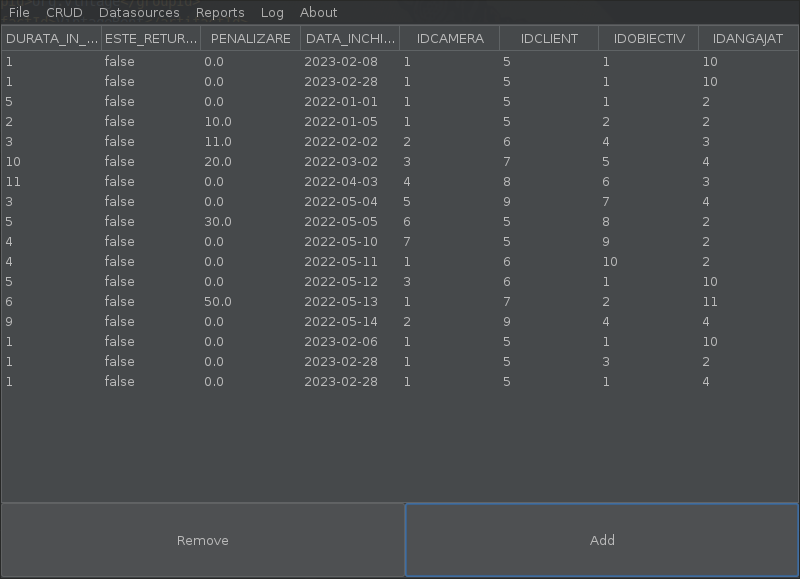
\includegraphics[width=\linewidth]{program.png}
    \caption{Main GUI}
    \label{fig:maingui}
\end{figure}

Pentru tema am folosit \textbf{com.formdev.flatlaf} si am initializat \textbf{FlatDarkLaf}. Mai jos este codul dependentei din \textbf{pom.xml}.
\begin{center}
    \begin{lstlisting}[language=pom]
    <dependency>
        <groupId>com.formdev</groupId>
        <artifactId>flatlaf</artifactId>
        <version>3.0</version>
    </dependency>
    \end{lstlisting}
\end{center}

\paragraph{} Interfata grafica principala consta dintr-o \textbf{bara de meniu} si un \textbf{gridbaglayout} in care este pus un \textbf{JTable} si doua butoane de \textbf{remove} si \textbf{add}.

\paragraph{Bara de meniu} are mai multe elemente:
\begin{enumerate}
    \item File - de aici se poate iesi din program
    \item CRUD - contine tabelele pe care se poate lucra si se va face update la alegerea oricarui tabel, evident ca folosind datele din data sourceul selectat
    \item Datasources - contine sursele de date disponibile si se va face update la alegerea oricarei surse de date
    \item Rapoarte - contine rapoartele
    \item Log - contine un item pentru afisarea logurilor
    \item About - afiseaza informatii despre program
\end{enumerate}

\paragraph{JTable} este evident continut intr-un \textbf{JScrollPane} si are un data source dat prima data de \textbf{Rent} pentru \textbf{read}. Contine un eveniment de setare a valorii in caz de \textbf{update}. Unele tabele pot fi sortate, altele nu, depinde de la caz la caz. Oricum, chiar si in cele care pot fi  sortate, operatiunile decurg normal, deoarece se obtine indexul corect al liniei si coloanei.

\paragraph{Butonul remove} va sterge randul selectat atunci cand este apasat.

\paragraph{Butonul add} va deschide o fereastra personalizata in functie de fiecare tabela in parte. In continuare voi vorbi despre ferestrele de adaugare.

\subsection[Add]{Add}
\begin{figure}[ht]
    \centering
    \noindent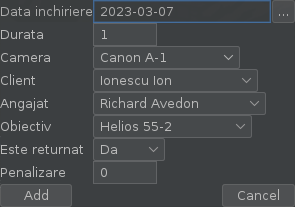
\includegraphics[scale=0.6]{addgui.png}
    \caption{Add GUI}
    \label{fig:addgui}
\end{figure}

\paragraph{} Ferestrele de adaugare sunt facute in functie de fiecare clasa in parte. Ca element comun toate contin un \textbf{gridbaglayout}, un buton de adaugare si unul de iesire, precum si mai multe JLable-uri.

\paragraph{} Elementele optionale pe care le pot contine sunt:
\begin{enumerate}
    \item \textbf{JTextField} pentru text normal
    \item \textbf{JPasswordField} pentru parole
    \item \textbf{JComboBox} in cazul unei chei externe pentru alegerea in functie de informatiile din tabelul de legatura
    \item \textbf{JDatePickerImpl} pentru alegerea datelor calendaristice
\end{enumerate}

\paragraph{} Daca primele doua sunt evidente, pentru celelalte doua voi detalia.

\paragraph{JComboBox} reprezinta un combo box pentru a alege datele in functie de ce se afla in tabelul de legatura. Ca element, am creat \textbf{org.gui.custom.ComboItem} pentru a putea opera cu o cheie si o valoare. Cheia reprezinta valoarea campului de legatura, iar valoarea ceea ce se va afisa.

\paragraph{JDatePickerImpl} reprezinta un date picker de la \textbf{org.jdatepicker.jdatepicker}. Acesta poate vine cu un panou care se afiseaza dinamic pentru alegerea datei calendaristice. Codul pentru dependenta adaugat in \textbf{pom.xml} este:
\begin{center}
    \begin{lstlisting}[language=pom]
<dependency>
    <groupId>org.jdatepicker</groupId>
    <artifactId>jdatepicker</artifactId>
    <version>1.3.4</version>
</dependency>
    \end{lstlisting}
\end{center}

\subsection[Rapoarte]{Rapoarte}
\paragraph{Raport clienti} reprezinta raportul in care se pot afisa date despre ce a inchiriat un client. Acesta contine un \textbf{JComboBox} pentru a alege clientul cu un eveniment de schimbare astfel incat sa se actualizeze automat datele din \textbf{JTable}-ul de mai jos. De asemenea, contine si un buton de exit.

\paragraph{Raport vanzari per format} reprezinta raportul in care se afiseaza date despre vanzarile pentru formatul ales.


\subsection[Log]{Log}
\begin{figure}[H]
    \centering
    \noindent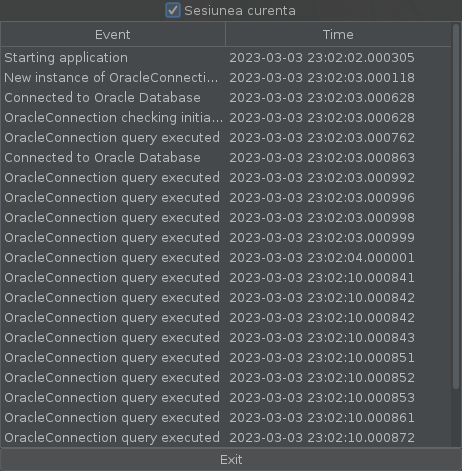
\includegraphics[scale=0.6]{loggui.png}
    \caption{Log GUI}
    \label{fig:loggui}
\end{figure}
\paragraph{} Contine logurile sesiunii curente, dar si un \textbf{JCheckBox} astfel incat sa poata fi vazute toate. Acestea sunt scrise intr-un fisier CSV si preluate de acolo intr-un \textbf{JTable} continut intr-un \textbf{JScrollPane}.

\section[Conexiunea la data sourceuri]{Conexiunea la data sourceuri}

\begin{figure}[ht]
    \centering
    \noindent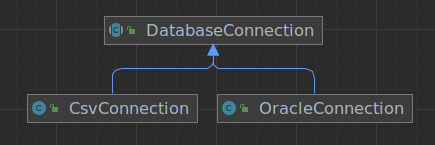
\includegraphics[scale=0.7]{diagramadb.png}
    \caption{Diagrama claselor care se ocupa de relatia cu data sourceurile}
    \label{fig:diagramadb}
\end{figure}


\paragraph{Clasa abstracta} \textbf{org.database.DatabaseConnection} contine atributele si metodele necesare de implementat de catre \textbf{OracleConnection} si \textbf{CsvConnection} care o mostenesc. 

\paragraph{} Deoarece clasa nu poate fi initializata, ea functioneaza si pe post de \textbf{factory} pentru celelalte clase. Astfel ca e nevoie de un \textbf{public enum DatabaseType} pentru a da tipul de data source care se doreste in metoda \textbf{getInstance}. De asemenea, pentru ca celelalte 2 clase sunt de tip \textbf{singleton}, aceasta are un pool de conexiuni pe care il completeaza pe masura ce se creaza instante din clasele noi. Pool-ul este in \textbf{protected static ArrayList<DatabaseConnection> instances}.

\paragraph{OracleConnection} este clasa care mosteneste DatabaseConnection si implementeaza metodele acesteia de conectare la baza de date si manipulare a datelor. Evident ca toate sunt in functie de cerintele necesare sistemului de gestiune a bazelor de date Oracle careia ii trimite queryuri. Aceste queryuri nu sunt protejate la un atac de tip sql injection, ramane in lista de todo de implementat o astfel de protectie.

\paragraph{CsvConnection} este clasa care, de asemenea, mosteneste DatabaseConnection si implementeaza metodele de manipulare a fisierelor Csv. Aici sunt cateva particularitati.

\paragraph{} In primul rand, fisierele Csv nu au integritate referentiala, iar programul nu este un sistem de gestiune a lor asemanator cu unul al unei baze de date. Asadar, utilizatorul trebuie sa fie atent la modificarea fisierelor astfel incat sa nu strice integritatea lor.

\paragraph{} Pentru manipularea datelor am folosit \textbf{com.opencsv.opencsv}. Codul din pom.xml pentru aceasta dependenta este urmatorul:

\begin{center}
    \begin{lstlisting}[language=pom]
<dependency>
    <groupId>com.opencsv</groupId>
    <artifactId>opencsv</artifactId>
    <version>5.7.1</version>
</dependency>
    \end{lstlisting}
\end{center}

\paragraph{} Deoarece apar diferente fata de bazele de date care au deja rezultate implementate ca \textbf{ResultSet}, am folosit \textbf{com.mockrunner.mockrunner-jdbc} pentru a simula acest tip de date astfel incat metodele sa aiba o valoare returnata standard. Codul din pom.xml pentru acesta este urmatorul:

\begin{center}
    \begin{lstlisting}[language=pom]
<dependency>
    <groupId>com.mockrunner</groupId>
    <artifactId>mockrunner-jdbc</artifactId>
    <version>2.0.1</version>
</dependency>
    \end{lstlisting}
\end{center}

\paragraph{} Deoarece clasa este folosita si de serviciul de audit, aceasta impelmenteaza cateva metode care nu se regasesc in celelalte conexiuni. Aceste metode sunt \textbf{insertNoLog} care face inserarea fara a scrie acest lucru in loguri (altfel s-ar crea o bucla infinita) si \textbf{readAllNoLog} care citeste un fisier de log, la fel fara a scrie acest lucru in loguri. In serviciul de audit se face un upcasting catre aceasta clasa la instanta de DatabaseConnection pentru a-i folosi metodele specifice.

\paragraph{} Pentru ca resursele pot sa nu fie alocate deja, am facut un hack si am inclus un fisier \textbf{CSV/mock.csv} careia sa-i ia calea in caz ca doreste sa creeze un fisier care inca nu exista al unei tabele. Acest comportament poate fi observat in metoda \textbf{createAndINsertDynamically}.

\section[Modele]{Modele}
\subsection[Model]{Model}
\paragraph{}Clasa abstracta \textbf{Model} contine ceea ce este necesar pentru a crea un model concret:
\begin{enumerate}
    \item Atributul de instanta pentru a fi singleton
    \item Atributul de tip de baza de date pentru conectare
    \item Atributul de nume cu getter si setter
    \item Metoda statica de preluare a instantei pentru a asigura proprietatea de singleton
    \item Metoda de setare a unui tip de baze de date
    \item O clasa interioara statica si abstracta denumita \textbf{AbstractInnerModel} unde vor fi puse atributele necesare fiecarui model atunci cand le preia din data source
\end{enumerate}

\subsection[ModelList]{ModelList}
\paragraph{} Clasa \textbf{ModelList <T extends Model.AbstractInnerModel>} contine un template pentru a limita tipul de date al listelor pe care le creaza la cel specificat, precum si un atribut privat de tip \textbf{List<T>} unde va stoca lista.
\paragraph{} Are 3 constructori, unul parametrizat pentru initializarea listei cu o lista data, altul neparametrizat care initializeaza lista implicit cu un ArrayList, iar altul parametrizat cu un boolean pentru a initializa cu un SortedArrayList.
\paragraph{} Contine o clasa denumita \textbf{SortedArrayList<T>} care mosteneste ArrayList si face override pe metodele de adaugare, actualizare si stergere specifice astfel incat sa poata pastra lista sortata.
\paragraph{} Contine mai multe metode de a manipula lista continuta.

\subsection[LinkModelToDatabase]{LinkModelToDatabase}
\paragraph{} Contine mai multe metode necesare unui model pentru a lucra cu baza de date (CRUD), precum si o metoda specifica aplicatiei pentru a scrie datele din baza de date intr-un fisier CSV.

\paragraph{} In semnatura sa, \textbf{public interface LinkModelToDatabase<T extends ModelList, U extends Model.AbstractInnerModel>} apar 2 templateuri, unul pentru a fi sigur ca este de tip ModelList, iar altul pentru a fi sigur ca extinde clasa de campuri continuta de fiecare model in parte.

\subsection[*Model]{*Model}
\paragraph{} Prin acest lucru definesc orice model. Deoarece modelele functioneaza pe acelasi principiu, dar cu o alta multime de campuri mapate din data source, este de preferat sa fac o descriere generala pentru a putea implementa orice alt model pe viitor.

\begin{figure}[ht]
    \centering
    \noindent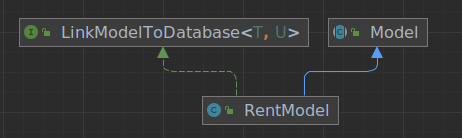
\includegraphics[scale=0.7]{rentmodel.png}
    \caption{Diagrama RentModel}
    \label{fig:rentmodel}
\end{figure}

\paragraph{} Clasele modelelor concrete, extind clasa Model si implementeaza interfata LinkModelToDatabase oferindu-i valori corecte pentru template. Un exemplu de astfel de semnatura este: \textbf{public class RentModel extends Model implementsLinkModelToDatabase < ModelList <RentModel.InnerRentModel>, RentModel.InnerRentModel>}.

\paragraph{} Contin o clasa interioara statica ce extinde AbstractInnerModel in care se definesc campurile care se vor utiliza.
\paragraph{} Mentionez in continuare modalitatea standard de implementare pentru cele mai importante metode:
\begin{enumerate}
    \item getTableModel defineste un array de string-uri cu coloanele si apoi creaza si returneaza un DefaultTableModel
    \item transferToModelList transfera un ResultSet in ModelList-ul corespunzator
    \item getData() incepe prin a defini un map cu denumirea generala a tabelelor si locul unde se pot gasi in baza de date. Apoi preia ResultSet-uri din mai multe tabele, iar in afara de cel principal, pe celelalte le pune intr-un Map<Integer, String> pentru a avea cheia primara si valoarea care se doreste extrasa. Apoi, pentru fiecare inregistrara din tabela principala, va mapa datele obtinute din celelalte tabele si va popula ModelList-ul. Am ales aceasta metoda deoarece este comuna atat bazelor de date relationale, cat si fisierelor csv.
    \item updateData primeste un rand de actualizat sub forma unui ModelList si mapeaza pe baza lui toate campurile ce pot fi actualizate, apoi intr-o mapare separata va pune campurile care definesc cheia primara. La sfarsit ia obiectul data sourceului si apeleaza functia de update
    \item deleteRow preia un rand sub forma unui ModelList si creaza clauza where specifica stergerii pe care o trimite mai departe obiectului data sourceului si apeleaza functia delete.
    \item throwIntoCsv verifica daca are o conexiune la o baza de date, apoi ia pe rand toate rezultatele, inclusiv din metadatele ResultSet-ului coloanele, apoi apeleaza metoda de creare si inserare din CsvConnection
    \item insertRow preia un model ce extinde AbstractInnerModel si creaza o lista de valori de forma \textbf{List<Pair<String, String>{}>} in care adauga pe rand valorile. Daca in spate modelul are o cheie primara care se incrementeaza, acesta exclude valoarea noua a cheii primare.
\end{enumerate}

\section[Serviciul de audit]{Serviciul de audit}
\paragraph{CsvLogger} este numele serviciului de audit care scrie logurile intr-un fisier csv. Acesta extinde \textbf{java.util.logging.Logger} si este de tip singleton. Are un constructor privat si singurul mod in care poate fi creata instanta este prin metoda statica \textbf{getInstance}.

\paragraph{Metoda de scriere} log primeste un mesaj de tip String si il scrie in fisier.

\paragraph{Metodele de citire} readLog() si readLogToday() citesc intreg fisierul de log, respectiv doar cel de la inceputul sesiunii si pana acum si corespund optiunilor din interfata grafica. Ambele returneaza un \textbf{Pair<List<String>, List<List<String>{}>{}>} cu headerul, respectiv corpul fisierului.

\section[Rapoarte]{Rapoarte}
\paragraph{} Rapoartele si alte actiuni pot fi accesate direct din \textbf{org.actions.MainService}.

\subsection[Raport client]{Raport client}
\paragraph{} Acesta primeste un intreg care reprezinta ID-ul clientului si un tip de baza de date. Returneaza un \textbf{Map<String, String>} reprezentand maparea tuturor datelor obtinute. Ca mentiune separata, pentru a numara camerele distincte am optat pentru o integrare comuna intre CSV si bazele de date, asa ca am efectuat o singura interogare si le pun intr-un \textbf{HashSet<Integer>}, iar apoi extrag dimensiunea lui.

\subsection[Raport vanzari per format]{Raport vanzari per format}
\paragraph{} Acesta primeste un intreg care reprezinta ID-ul formatului si un tip de baza de date. Returneaza un \textbf{Map<String, String>} reprezentand maparea tuturor datelor obtinute. Pentru a face ordonarea preturilor foloseste un \textbf{PriorityQueue<Double>} initializat ca \textbf{new PriorityQueue<> (Collections.reverseOrder())}. Pentru clienti foloseste un \textbf{HashSet<Integer>} din aceleasi motive ca la raportul de clienti.

\section[Clase ajutatoare]{Clase ajutatoare}
\subsection[Pair<T, U>]{Pair<T, U>}
\paragraph{} Deoarece in Java nu exista un tip pair nativ, am scris o clasa care foloseste doua templateuri, T si U, si creaza o pereche mapand obiectele pe atributele first si second. Acesta sunt publice, dar se pot accesa si prin getteri.

\subsection[ModelInit]{ModelInit}
\paragraph{} Aceasta clasa se ocupa cu initializarea modelului pentru fisierele CSV corespunzatoare tabelelor. Daca acestea nu sunt gasite, programul va lua pe rand tabelele din baza de date si le va arunca datele in fisiere CSV corespunzatoare pentru ca modelele sa functioneze si cu acest tip de fisiere.

\section[Resurse]{Resurse}
\paragraph{}Folderul de resurse este impartit in:
\begin{enumerate}
    \item CSV cu fisierele CSV
    \begin{enumerate}
        \item Fisierele corespunzatoare tabelelor
        \item Folderul Log
    \end{enumerate}
    \item META-INF cu manifestul
    \item Migrations cu fisierul sql care este rulat pentru a popula baza de date
    \item Spalsh cu imaginea pentru spalsh screen
\end{enumerate}

\section[Workflow GitHub]{Workflow GitHub}
\paragraph{} Actiunea de publicare a unei versiuni noi pe GitHub are urmatorii pasi:
\begin{enumerate}
    \item Checkout
    \item Setare Java 17 Oracle
    \item Preluarea versiunii proiectului cu ajutorul Maven din pom.xml
    \item Buildul facut de Maven
    \item Uploadul artefcatului de realease (fisierul .jar) in mediul actiunii
    \item Crearea pachetului de release
    \item Atasarea artefactului de release la pachet
\end{enumerate}

\paragraph{} Toate aceste lucruri se pot face atat manual cat si la fiecare push pe main. De aceea pentru fiecare versiune noua se va lucra pe un branch separat.

\paragraph{} Fisierul de workflow se afla in \textbf{./.github/workflows/main.yml}.

\section[Alte mentiuni despre cod]{Alte mentiuni despre cod}
\paragraph{} Codul se refera la un produs MVP de gestionare a unui magazin de vanzare a camerelor foto vintage. Pe parcurs am spus ce poate fi imbunatatit, iar in fisierul {\color{blue}\url{https://github.com/fredtux/VintageRent/blob/main/README.MD}} se pot gasi mai multe informatii referitoare la indeplinirea cerintelor.


\end{document}